\documentclass{minimal}

\usepackage{amsmath}
\usepackage{amssymb}
\usepackage{bm}
\usepackage{graphicx}

\DeclareMathOperator*{\argmax}{argmax}
\DeclareMathOperator*{\argmin}{argmin}

\begin{document}

\textbf{Linear classifiers}

Linear discriminant analysis (LDA)

Logistic regression

Support vector machine (SVM)

\medskip

\textbf{LDA}

Assume classes are multivariate Gaussian with common covariance matrix $\mathbf{\Sigma}$

It can be shown that under these assumptions the decision boundary between any
two classes is linear, i.e. a hyperplane in $\mathbb{R}$.

\smallskip

$w$ is a weight vector that defines a projection into a 1-dimensional subspace.
Then, in that sub-space, we set a threshold $t$ as the boundary between the two
classes. 

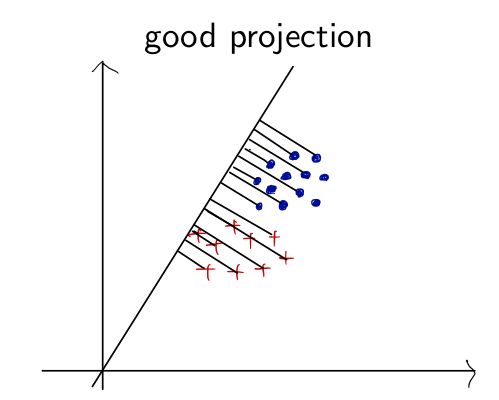
\includegraphics[scale=0.25]{lda}

Fisher's optimal projection: maximize between-class variance relative
to within-class variance. In other words: projected class centroids are far
apart, projected data are close to centroids.

$$
\hat{w} = \argmax_{w \in \mathbb{R}^d} \frac{w'\mathbf{B}w}{w'\mathbf{W}w}
$$

$$
\mathbf{B} = \sum_c (\bm{\mu}_c - \bar{\mathbf{x}}) (\bm{\mu}_c -
\bar{\mathbf{x}})'
$$
$$
\mathbf{W} = \sum_c \sum_{i \in c}(\mathbf{x}_i - \bm{\mu}_c) (\mathbf{x}_i -
\bm{\mu}_c)'
$$

\smallskip

Because $w$ is invariant to rescaling, we can choose $w$ such that
$w'\mathbf{W}w=1$, leading to:

$$
w^* = \argmax_w w'\mathbf{B}w 
$$
\begin{center}
s.t.
\end{center}
$$
w'\mathbf{W}w=1
$$

This is a generalized eigenvalue problem, with $w$ given by the largest
eigenvalue of $\mathbf{W}^{-1}\mathbf{B}$

\smallskip

If we assume Gaussian class densities and common covariance matrix
$\mathbf{\Sigma}$, then LDA is optimal (equivalent to Bayes).

\medskip

\textbf{Interlude: Lagrangian optimization}

Suppose that we have a standard optimization problem with $m$ inequality and/or
$p$ equality constraints:

\smallskip

Minimize $f_0(x)$

s.t. $f_i(x) \leq 0, \quad i=1...m$

$h_i(x)=0, \quad i = 1...p$

The Lagrangian is:
$$
L(x, \lambda, v) = f_0(x) + \sum_{i=1}^m \lambda_if_i(x) + \sum_{i=1}^p v_i
h_i(x)
$$

The dual function is the minimum value of the Lagrangian over $x$:
$$
g(\lambda, v) = \inf_x L(x, \lambda, v)
$$

This function is concave, even if the original problem is not convex. It also is
always less than or equal to the original objective function evaluated at its
optimal value. Putting these together, if we maximize $\lambda$ and $v$ in the dual, it is the same
as minimizing $x$ in the primal.

\smallskip

Slater's condition: if the primal and dual are feasible, then the gap is zero.

\smallskip

Complementary slackness: if a variable is positive, then the associated dual
constraint must be binding. If a constraint fails to bind, then the associated
variable must be zero.

\medskip

\textbf{Logistic}

Same as usual. Estimate using MLE. Can add a regularizer. Often outperforms LDA
because it doesn't have squared error (bad). Example:

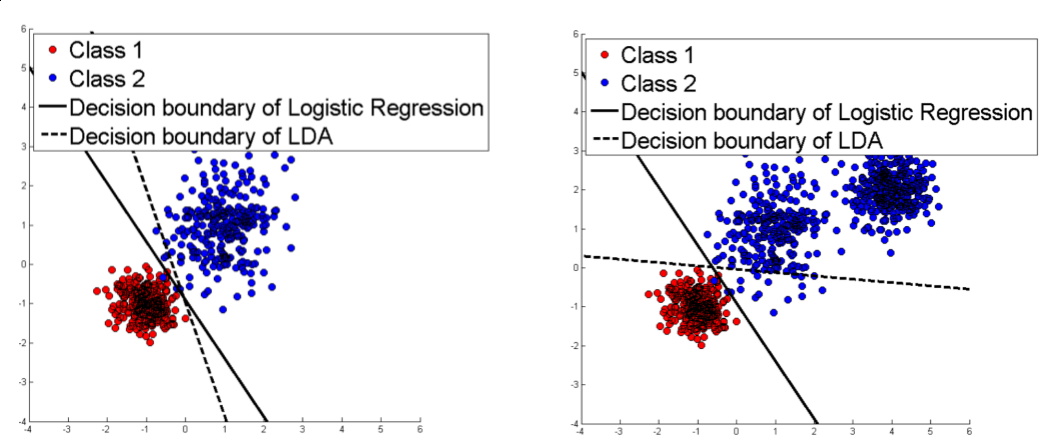
\includegraphics[scale=0.25]{log}

\medskip

\textbf{SVM}

\smallskip

\textit{Hard margin (linearly separable data)}

Suppose we have labels $Y_i \in \{-1,1\}$ and data $X_i$. 

We want to construct a decision hyperplane $\langle w, X \rangle + b= 0$. $w$ is
a weight vector that we apply to $X$. If for a particular observation $\langle w, X_i \rangle + b < 0$, we
classify as $Y_i=-1$. Similarly, if $\langle w, X_i \rangle + b > 0$, we
classify it as $Y_i = 1$

Notation note:
$$b + \langle w, x \rangle = \mathbf{w}^T\mathbf{X} + b = \sum w_ix_i + b$$ 

What makes a good hyperplane? Assuming linear separability, a criterion is that
it maximizes the minimum distance from the data points to the hyperplane. The
distance of a point $x_i$ to a hyperplane $w'x + b$ is:

$$
\frac{|w'x_i + b|}{||w||}
$$

So, we might construct a good hyperplane by trying to maximize the distance to
the closest point:

$$
\max_{w, b} \min\{\frac{|w'x_i + b|}{||w||}\}
$$

We also want to make sure that it classifies correctly, so we add the
below constraint. 

$$
s.t. \quad Y_i(\langle w, x_i \rangle + b) \geq 1 \quad \forall i
$$

A problem, however, is that this won't have a unique solution because we can
scale the problem by some constant $\gamma$ and obtain identical results. We get
around this by stipulating that the hyperplane must be \textit{canonical}
to $X$, which means that the distance between the hyperplane and the closest
point is unity.

$$
\min_{1 \leq i \leq n} |\langle w, x_i \rangle + b| = 1
$$

Since we now know that the distance between the hyperplane and the point closest
to the hyperplane is unity, the problem becomes: 

$$
\max_{w, b}\frac{1}{||w||}
$$
$$
s.t. \min_{1 \leq i \leq n} |\langle w, x_i \rangle + b| = 1
$$
$$
\quad Y_i(\langle w, x_i \rangle + b) \geq 1 \quad \forall i
$$

Maximizing the above function is equivalent to minimizing $||w||$. We will add
some other stuff to the problem to make later work easier.

$$
\min_{w, b}\frac{1}{2}||w||^2
$$
$$
s.t. \min_{1 \leq i \leq n} |\langle w, x_i \rangle + b| = 1
$$
$$
\quad Y_i(\langle w, x_i \rangle + b) \geq 1 \quad \forall i
$$


This is a quadratic function with linear constraints, aka quadratic programming.
The Lagrangian is:
$$
L(b, w, \alpha) = \frac{1}{2}||w||^2 + \sum_{i=1}^n \alpha_i [1 - Y_i(\langle
w, x_i \rangle + b)]
$$

We need the minima to compute the dual. We find them by taking the derivative
and setting equal to 0:

$$
\nabla_w = 
\nabla_w \left( \frac{1}{2}||w||^2 \right) + 
\nabla_w \left(\sum_{i=1}^n \alpha_i \right) - 
\nabla_w \left( \sum_{i=1}^n \alpha_i Y_i \langle w, x_i \rangle \right) - 
\nabla_w \left( \sum_{i=1}^n \alpha_i Y_i b \right)
= 0
$$
$$
w = \sum_{i=1}^n \alpha_i Y_i x_i
$$
$$
\frac{\partial L}{\partial b} = \frac{\partial}{\partial b}
\left( \frac{1}{2}||w||^2 \right) + \frac{\partial}{\partial b}
\left(\sum_{i=1}^n \alpha_i \right) - \frac{\partial}{\partial b}\left( \sum_{i=1}^n \alpha_i Y_i \langle
w, x_i \rangle \right) - \frac{\partial}{\partial b} \left( b \sum_{i=1}^n
\alpha_i Y_i \right)
=0
$$
$$
\sum_{i=1}^n \alpha_i Y_i = 0
$$

We plug them into the Lagrangian to obtain the dual. By
definition, $||v||^2 = \langle v, v \rangle$. So:

$$
\frac{1}{2} ||w||^2 = \frac{1}{2} \langle w, w \rangle = 
\frac{1}{2} \langle \sum_{i=1}^n \alpha_i Y_i x_i, \sum_{j=1}^n \alpha_j Y_j x_j \rangle
$$

The $\alpha$ and $Y$ are just scalars and so we can pull them out:

$$
= \frac{1}{2} \sum_{i=1}^n \sum_{j=1}^n \alpha_i \alpha_j Y_i Y_j \langle x_i, x_j \rangle
$$

Now we factor out the right hand side:

$$
\sum_{i=1}^n \alpha_i [1 - Y_i(\langle w, x_i \rangle + b)] = \sum_{i=1}^n
\alpha_i [1 - Y_i \langle w, x_i \rangle - Y_i b]
$$
$$
= \sum_{i=0}^n \alpha_i - \sum_{i=0}^n \alpha_i Y_i \langle w, x_i \rangle -
b \sum_{i=0}^n \alpha_i Y_i
$$

We know that:

$$
b \sum_{i=0}^n \alpha_i Y_i = b \times 0 = 0
$$

Now let's plug $w$ into the middle term:

$$
\sum_{i=0}^n \alpha_i Y_i \langle \sum_{j=0}^n \alpha_j Y_j x_j, x_i \rangle
$$

Again we can pull out the scalars:

$$
= \sum_{i=0}^n \sum_{j=0}^n \alpha_i \alpha_j Y_i Y_j \langle x_i, x_j \rangle
$$

We recombine everything to form the dual:

$$
q(\alpha) = \frac{1}{2} \sum_{i=1}^n \sum_{j=1}^n \alpha_i \alpha_j Y_i Y_j
\langle x_i, x_j \rangle + \sum_{i=1}^n \alpha_i - 
\sum_{i=0}^n \sum_{j=0}^n \alpha_i \alpha_j Y_i Y_j \langle x_i, x_j \rangle
$$

$$
= \sum_{i=1}^n \alpha_i - \frac{1}{2} \sum_{i=0}^n \sum_{j=0}^n \alpha_i \alpha_j Y_i Y_j \langle x_i, x_j \rangle
$$

Hence, the dual problem is:

$$
\max_{\alpha \in \mathbb{R}^n} 
\sum_{i=1}^n \alpha_i - \frac{1}{2} \sum_{i=0}^n \sum_{j=0}^n \alpha_i \alpha_j Y_i Y_j \langle x_i, x_j \rangle
$$
$$
s.t. \quad \alpha_i \geq 0 \quad \forall i
$$
$$
\quad \sum_{i=0}^n Y_i \alpha_i = 0
$$

The first constraint corresponds to our ``correctness'' constraint in the
objective. The second constraint is a ``balance'' constraint: that the distances
from points to the hyperplane must balance each other out.

Both the primal and dual are feasible, so the dual gap is 0 and solving the dual is
equivalent to solving the primal. 

Looking at this dual gives us some interesting properties. Complementary slackness 
says that if a variable is positive,
then the associated dual constraint must be binding; conversely, if a constraint
fails to bind, then the associated dual variable must be zero. In the primal, we
had the constraint $Y_i(b + \langle w, x_i \rangle)\geq 1$, which is the same as
$1 - Y_i(b + \langle w, x_i \rangle) \leq 0$. If for primal constraint $1 - Y_i(b + \langle w, x_i
\rangle) = 0$, i.e. $x_i$ lays exactly on the margin, then the dual variable
$\alpha_i > 0$. In other words, only points laying on the
margin---\textit{support vectors}---determine the
separating hyperplane. 

This definitely helps our robustness: 
variation of training points won't change our decision hyperplane unless the
points happen to fall on the margin. 

It also can help our computation if we have
some heuristics to determine before computing $w$ what are some likely support
vectors.

In essence, specifying a hyperplane---a function of a simple form $w'x$---helps
us control $d$ and avoid the curse of dimensionality. The support vector
property helps us control $n$.

To determine $b$, we average $Y_i - \langle w, x_i \rangle$ over all $i$ with
$\alpha_i > 0$.

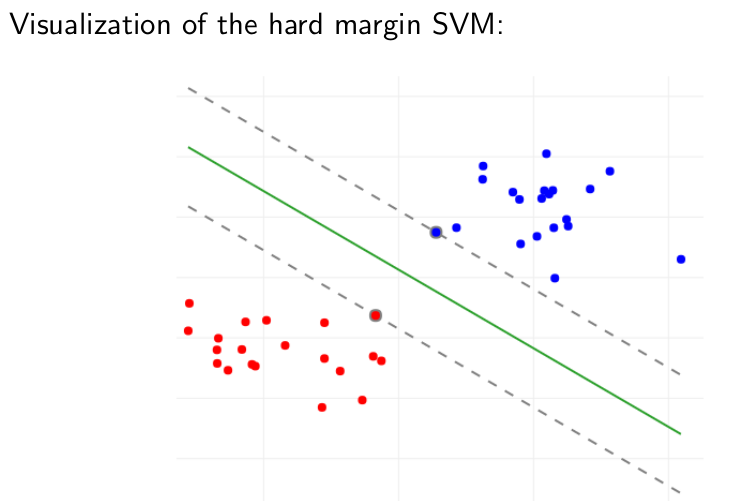
\includegraphics[scale=0.25]{svm1}

\medskip

\textit{Soft margin}

The above approach may not always be possible (since it requires linear
seperability) or desirable (since it may lead to overfitting). So, we have the
alternative soft margin approach. We introduce slack variables, as well as a 
cost parameter to control them. The problem becomes:

$$
\min_{w \in \mathbb{R^d}, b \in \mathbb{R}, \xi \in \mathbb{R}^n} 
\frac{1}{2} ||w||^2 + C \frac{1}{n} \sum_{i=1}^n \xi_i
$$
$$
s.t. \quad Y_i(\langle w, x_i \rangle + b) \geq 1 - \xi_i \quad \forall i
$$
$$
\quad \xi_i \geq 0 \quad \forall i
$$

We also can view this problem through the lens of ERM. Let's say we obtain an
optimal solution $w^*, b^*, \xi^*$. 
Then, it makes sense that:
$$
\xi_i^* = \max(0, 1 - Y_i(\langle w, x_i \rangle + b)) 
$$

We now can recharacterize the problem as:
$$
\min_{w, b} C \frac{1}{n} \sum_{i=1}^n \max(0, 1 - Y_i(\langle w, x_i \rangle +
b)) + \frac{1}{2}||w||^2
$$

This is equivalent to:
$$
\min_{f \in \mathcal{F}} \frac{1}{n} \sum_{i=1}^n L(Y_i f(X_i)) + \lambda
||w||^2
$$

Where $\mathcal{F}$ is the linear hypothesis class, $L$ is the hinge loss, and
$\lambda=\frac{1}{2C}$

\medskip

Anyways, the Lagrangian thus is:
$$
L(w, b, \xi, \alpha, \beta) = 
\frac{1}{2} ||w||^2 + 
C \frac{1}{n} \sum_{i=1}^n \xi_i +
\sum_{i=1}^n \alpha_i(1 - \xi_i - Y_i (\langle w, x_i \rangle + b)) -
\sum_{i=1}^n \beta_i \xi_i
$$

Taking the gradient or partial derivative w/r/t $w, b, \xi$ yields:
$$
w = \sum_{i=1}^n \alpha_i Y_i x_i
$$
$$
\sum_{i=1}^n \alpha_i Y_i = 0
$$
$$
\sum_{i=1}\beta_i = \frac{C}{n} - \sum_{i=1}^n \alpha_i \to \beta_i = \frac{C}{n} - \alpha_i
$$

Since $\beta_i \geq 0$, we can deduce an upper limit for $\alpha_i$
$$
0 \leq \alpha_i \leq \frac{C}{n} \quad \forall i
$$

This results in:

$$
\max_{\alpha \in \mathbb{R}^n} 
\sum_{i=1}^n \alpha_i - \frac{1}{2} \sum_{i=0}^n \sum_{j=0}^n \alpha_i \alpha_j Y_i Y_j \langle x_i, x_j \rangle
$$
$$
s.t. \quad 0 \leq \alpha_i \leq \frac{C}{n} \quad \forall i
$$
$$
\quad \sum_{i=0}^n Y_i \alpha_i = 0
$$

All our previous observations about support vectors still hold.

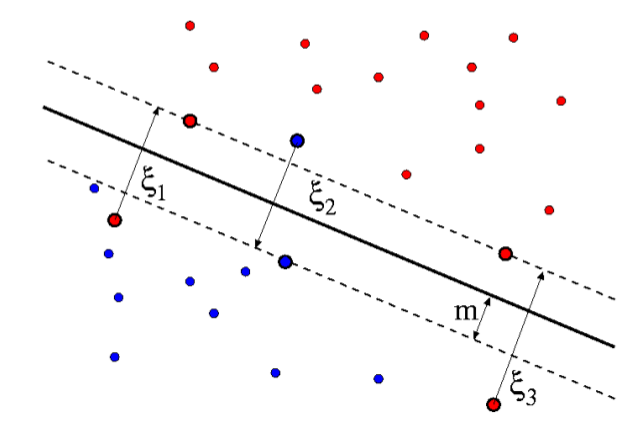
\includegraphics[scale=0.25]{soft.png}
\end{document}



